\documentclass[11pt]{article}
\usepackage[margin=2.7cm]{geometry}
\usepackage{amsmath,amssymb}
\usepackage{graphicx}
\usepackage{booktabs}
\usepackage[hidelinks]{hyperref}
\usepackage{xeCJK}
\setCJKmainfont{Hiragino Mincho ProN}

\newcommand{\Myr}{\,\mathrm{Myr}}
\newcommand{\pc}{\,\mathrm{pc}}
\newcommand{\kms}{\,\mathrm{km\,s^{-1}}}
\newcommand{\lam}{\lambda}

\title{WAKE: 太陽近傍の来訪統計アトラス ---\\
Gaia DR3 実測運動学の上の到来統計・排除地図・フライバイ網\\[1ex]
\large (プレプリント --- 和文版。英語版が正文であり、本版は訳出である)}
\author{前田幸枝\thanks{独立研究者。AI システムの役割と検証プロトコル全体は
付録Bで開示する。この内部検証は人間の査読の代替ではない。}}
\date{2026年8月}

\begin{document}
\maketitle

\begin{abstract}
\noindent 太陽系は訪問済みのはずか。本論文は、太陽近傍の\textbf{実測}恒星運動学の
上で太陽系の来訪統計を初めて計算する: Gaia DR3(100 pc 以内の 6 次元位相空間
データを持つ 56{,}286 星)の接近統計に、Carroll-Nellenback らの探査機型・進入駆動
規約の入植動力学を重ねる。寄与は一つのカタログの上の三層である。
(1)\textbf{到来統計}: 会計規約を明示宣言した完備性補正・露出正規化の接近率。
公刊2陣営の会計規約を自データ上で再構成した結果、約2倍の分裂の主因は完備性補正が
対象とする母集団の違いであり、データ品質ではない。さらに値検疫・誤差検疫の双方を
すり抜ける第三の系統モード(Gaia RVS 暗端の視線速度アーティファクト — 接近率を
数倍膨張させうる)を同定し、接線速度整合検査を判別器として導入した。クリーン率は
FGK+早中期M母集団で $\lam(1\pc)=4.5^{+4.0}_{-2.7}\Myr^{-1}$。
(2)\textbf{排除地図}:「入植割合が $f^*$ を超えるなら、太陽系は過去 10\,Myr に
訪問済みのはず(沈黙は 95\% で棄却)」という条件付き言明。標準探査機航続距離
3.07 pc で $f^*=5.0\times10^{-3}$。三値の定理レイヤは、姉妹数学論文
(DOI 10.5281/zenodo.21955413)で証明された生存理論を輸入し、生存が定理保証される
領域・定理が沈黙する領域を分離し、完全モデルの絶滅定理は全域で存在しないことを
記録する。(3)\textbf{フライバイ網}: 接近通過の時変グラフ上に、推進剤最小の来訪
経路が窓内の全時刻で存在し、単一乗換の離脱予算は $\Delta v\simeq5.8\kms$ —
特定の星ではなく網の統計的性質である。すべての言明は宣言された母集団上の条件付き
確率文であり、判定不能領域は判定不能として報告する。これは測量であって証明ではない。
\end{abstract}

\tableofcontents

%======================================================================
\section{序論}\label{sec:intro}

太陽系は訪問済みのはずか。入植済みの系が銀河に存在し、最も安いチャネル ---
接近通過時に発進する遅く・小さく・古い探査機 --- で拡大するなら、太陽系に到達が
あったか否かは思弁の問題ではなく\textbf{実測運動学}の問題である: どの星がいつ、
どの頻度で航続距離内を通過したか、それを観測したサーベイの選択関数込みで。
本論文はその統計を Gaia DR3 上で計算し、入植動力学を重ねる。

本研究は来訪仮説検証プログラムの第三の枝である(ワープ級は ASTROGATION、高次元は
TESSERA が扱った。本枝は亜光速チャネルであり、太陽近傍の実運動学が決定的入力と
なる)。新規性の主張は意図的に狭い:\textbf{実カタログの接近統計への入植動力学の
重ね合わせ}である。第1層(接近統計)単体は確立した分野であり
\cite{bj18,bj22,gs01,fp26}、我々はそれを検証台として扱い、公刊アンカーの再現を
経てから新しいものを積む(第\ref{sec:prop}節)。入植動力学層の数学的基礎
(弾道運動点上の接触過程の生存・絶滅定理)は姉妹数学論文 \cite{wakemath} で
確立済みであり、ここではその仮定マップと保証だけを輸入する。全体を通じ、
プロジェクト憲法の規律が適用される: すべての出力言明は宣言された恒星母集団上の
条件付き確率文であり、データが判定できない領域は\textbf{判定不能}として報告し、
沈黙裡に埋めない。全体は測量であって証明ではない。

%======================================================================
\section{データ・選択・検疫}\label{sec:data}

\subsection{カタログと完備性}
Gaia DR3 の 100 pc 以内 6 次元標本 56{,}286 星を用いる \cite{gaiadr3}。選択は
DR3 RVS 選択関数 \cite{gaiaunlimited} の逆確率重み付け(IPW)で補正し、床値
$s_{\rm floor}=0.05$ を設ける: 選択確率が床値未満の星は重み上げせず
\textbf{判定不能母集団}(697 星)として報告する。補正後の母集団は明示的に
FGK+早中期M である。晩期M以深は全率から除外し判定不能と標識する
(率バウンド拡張は予約のみ)。

\subsection{5系統の検疫と第三の破れモード}\label{sec:bit5}
個別イベントの主張はアストロメトリ品質・固有運動 S/N・極端視線速度
($|RV|>550\kms$、確認済み超高速星の白名単経路付き)・視線速度誤差カット
($\sigma_{RV}>20\kms$ は個別判定除外・率には寄与)で防護する。

第\ref{sec:arrival}節の会計交差検証の過程で、値検疫・誤差検疫の双方をすり抜ける
\textbf{第三}の系統モードを同定した:\textbf{RVS 暗端の視線速度アーティファクト}
--- $G\gtrsim14$ で $|RV|=150$--$900\kms$ だが接線速度は円盤的な星である。真の
ハロー星は\textbf{両}成分がハロー運動学を示す。円盤的接線速度と極端視線速度の
組がアーティファクト署名である(DR3 RV 品質指針 \cite{katz23} 参照)。検疫
ビット5($G>13.5\wedge|RV|>150\kms$、1{,}323 星、閾値 $120/150/200\kms$ 走査で
クリーン成分安定)を追加し、超高速星ビットと同型運用とする: 個別イベント判定
除外・率は\textbf{両建て}報告(クリーン/込み)・接線速度整合検査による手動審査・
救済白名単(審査後も空 --- 上位 suspect は全てアーティファクト署名、例
$RV=-790\kms$ に $v_{\rm tan}=18\kms$)。未検疫なら sub-pc 接近率を約7倍膨張
させる(第\ref{sec:arrival}節)--- DR3 系接近研究への一般的な方法論的警告である。

%======================================================================
\section{伝播と検証}\label{sec:prop}

軌道は軸対称銀河ポテンシャル(MWPotential2014 級)の数値積分で伝播し、独立の
エピサイクル解析経路が定式化独立の対経路(ゲート G2)となる。検証アンカー
(ゲート G3)は新統計の主張前に公刊接近を再現する: ショルツ星
\cite{mamajek15,dupuy19}、GJ 710(我々の値 $1.294\Myr$・$0.0503\pc$ は
\cite{dlfm22} と一致。DR3 解析間の公刊値分裂は付録Aで中立に文書化)、接近頻度
アンカー \cite{bj18}。2種ポテンシャル監査(McMillan17 \cite{mcmillan17} を
スプライン表引き化し補間誤差自体も監査、相対 max $3.7\times10^{-5}$)が
ポテンシャル系統を抑え、遠時刻で2種差が測定不確かさを超える星は\textbf{実効
ホライズン}を短縮する(第3成分「$t_{\rm pot}$」)--- モデル不確かさを測定
不確かさと同格に、平均化ではなく判定不能として扱う。

各星は\textbf{個別ホライズン} $t_h$ を持つ: 位置不確かさ(視線速度誤差支配、
$1\kms\approx1\pc\Myr^{-1}$)が航続距離の半分を超える時刻である。統計は
\textbf{統制領域} $|t_{\rm ph}|\le t_h$ で計算し、ホライズン外のイベントは
図\ref{fig:lambdat}の判定不能の影 --- カタログの実測「証拠の地平線」--- を成す。
本研究中に G2 ゲートが発見・修正した実装欠陥2件(放物線精密化の係数と鋭極小の
破綻 --- 厳密な $d^2$ 補間で修復、G3 全アンカー再合格)は付録Bに開示する。

\begin{figure}[t]\centering
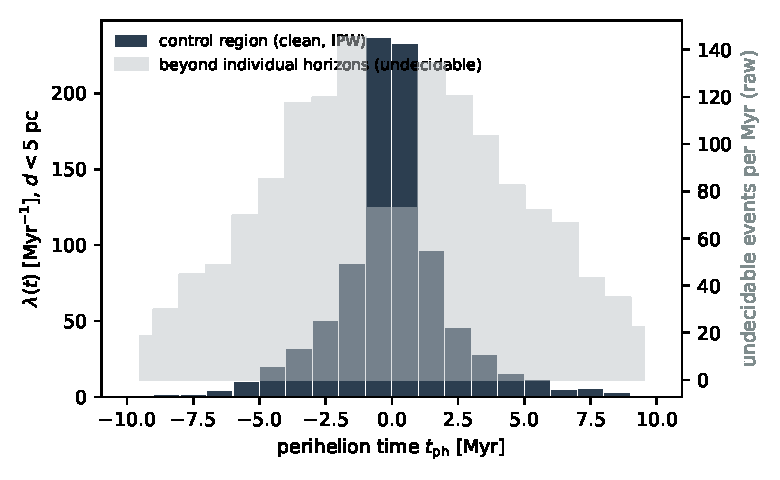
\includegraphics[width=.7\textwidth]{figs/fig1_lambda_t.pdf}
\caption{クリーン母集団の露出正規化到来率 $\lam(t)$(5 pc 以内、棒)と、個別
ホライズン外イベントの判定不能の影(灰)。包絡は Gaia DR3 の実測された証拠の
地平線である: 率はカタログが支持できる場所でのみ主張できる。再現:
\texttt{python3 src/wake\_p5/paper\_figs\_main.py}。}
\label{fig:lambdat}
\end{figure}

%======================================================================
\section{到来統計と接近率の会計}\label{sec:arrival}

\subsection{露出会計}
率とは計数を露出で割ったものであり、露出の選択は宣言すべき規約である。我々は
各星の寄与をその星自身の有効露出 $2\min(T,t_h)$ で正規化する。一律窓($1/2T$)は
窓が典型ホライズンを超えると率を希釈する。我々自身の初見値 $11.7\Myr^{-1}$
(1 pc)はまさにその規約(ホライズン無視・一律窓)から生じ、同規約下で厳密に
再現される --- 別の空ではなく、下方バイアスの会計である。露出正規化のクリーン率は
\[
\lam(1\pc)=4.49\;[1.78,8.50]\Myr^{-1},\quad
\lam(2\pc)=27.5\Myr^{-1},\quad
\lam(5\pc)=137.3\Myr^{-1}
\]
(1 pc は星ブートストラップ 95\% 区間。母集団: FGK+早中期M・IPW 補正。suspect
込み値はカタログに併記)。距離スケーリングは幾何的 $d^2$ 則から逸脱する
(1→2 pc で $6.1\times$、2→5 pc で $5.0\times$)--- 少数星支配の重い裾と IPW
重みの距離構造の反映である。

\subsection{一つのデータに三つの規約}
公刊の 1 pc 率2陣営 --- $19.7\pm2.2\Myr^{-1}$ \cite{bj18} と
$10.6\pm4.5\Myr^{-1}$ \cite{fp26} --- は会計規約(窓・露出・完備性対象・母集団)が
異なる。両規約を公刊本文から再構成し(本文から確定できなかった点 ---
\cite{bj18} 5件・\cite{fp26} 7件 --- は付録Aに中立に列挙)、単一データに三規約を
適用した:

\begin{center}
\begin{tabular}{lll}
\toprule
規約(我々のデータ上) & $\lam(1\pc)$ [$\Myr^{-1}$] & 公刊値 \\
\midrule
本機構(統制領域・IPW・星別露出) & $4.5^{+4.0}_{-2.7}$ & --- \\
BJ+18 再構成($G\le12.5$ 部分集合) & $23.7\pm2.6$ & $19.7\pm2.2$ \\
FP26 再構成(離散判定・信頼性カット) & $21.3$ & $10.6\pm4.5$ \\
\bottomrule
\end{tabular}
\end{center}

BJ 規約値はクリーンな DR3 データ上で再現される --- 残存 spurious アストロメトリが
分裂の主因である可能性は低い。FP26 との残差は第\ref{sec:bit5}節の暗端 RV
アーティファクトを除くと閉じる(明るい星のみの離散計数で $\simeq7.6$、彼らの
太陽値 $9.1$ と整合)。本再構成に基づけば、分裂の主因は\textbf{完備性補正が対象と
する母集団}である: \cite{bj18} はモック全恒星母集団へ補正し、\cite{fp26} は
窓因子以外を補正しない。整合的に、自データ上の二帳簿検査 --- 星別露出+IPW
(分母帳簿)対モック $C(t,d)$ 完備性地図(分子帳簿、付録C)--- は FGK+早中期M と
全恒星の間の実測\textbf{母集団の橋} $5.3\times$ を与え、\cite{bj18} のモック外挿が
含意する $\sim9\times$ と比較される --- モック型完備性補正の定量批評の基礎である。

\subsection{到来カタログと構造}
到来イベントカタログ($|t|\le13\Myr$ で中央値近日点 5 pc 以内の 2{,}197 星)は
既知の接近 --- HD 7977($0.037\pc$, $-2.76\Myr$)・GJ 710($0.052\pc$,
$+1.29\Myr$)--- を再現し、全検疫・ホライズン・両建て率メタデータを備える。
時間分解率 $\lam(t)$ に運動学的に整合な塊はなく(見かけの塊は全て単一星支配、
ペア $\Delta UVW\ge45\kms$)、接近対後退の小超過(相対 $+2.1\%$)は教科書的な
太陽向点双極子である(向点半球の接近割合 $75.4\%$ 対反向点 $24.1\%$)。標本
平均場の反射を引くと $+0.78\%$($1.9\sigma$)--- 空間構造なしと整合する。

%======================================================================
\section{排除地図}\label{sec:map}

\subsection{定義}
地図の条件付き言明は Poisson 訪問数で定義する:
\begin{equation}
N_{\rm vis} = f\cdot\frac{\langle \hat p\rangle}{f}\cdot\lam(R)\cdot
T_{\rm eff},\qquad
N_{\rm vis}\ge3\;\Longleftrightarrow\;P(\ge1\ \text{訪問})\ge95\%,
\label{eq:fstar}
\end{equation}
ここで $T_{\rm eff}=\max(0,\,10\Myr-R/v_p)$ は支持窓(探査機旅行時間を控除)、
$f$ は入植割合、$\langle\hat p\rangle/f$ はマーク場因子(定数場で 1、前線族は
実到来運動学で評価)、$\lam(R)$ は実測アンカー間の補間(1 pc 未満は $d^2$ 外挿・
フラグ付き、5 pc 超は判定不能)。クリーン率は物理的遭遇率の\textbf{下界}である
(探査機は Gaia の選択関数に従わない)ため「訪問済みのはず」領域は保守的に狭い。
母集団橋参考レイヤ($\times5.3$・モデル明示)と suspect 込みレイヤを併記する。

\begin{figure}[t]\centering
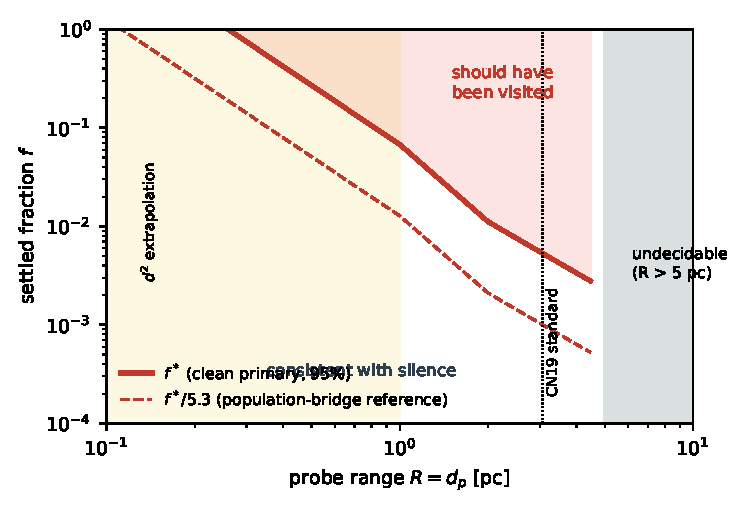
\includegraphics[width=.72\textwidth]{figs/fig2_exclusion_map.pdf}
\caption{$(R,f)$ 平面の排除地図($v_p=10\kms$・定数マーク場)。$f^*$(実線)の
上では宣言母集団に対し沈黙が 95\% で棄却される。破線は母集団橋参考。灰:
判定不能($R>5\pc$)。黄帯: $d^2$ 外挿。標準航続距離 $R=3.07\pc$ で
$f^*=5.0\times10^{-3}$。}
\label{fig:map}
\end{figure}

\cite{cn19} の標準航続距離($R=3.07\pc$)で
\[
\boxed{f^* = 5.0\times10^{-3}}
\]
--- \textbf{宣言母集団の 0.5\% 超が入植済み(かつ進入時発進)なら、太陽系は過去
10\,Myr に訪問済みのはず}である。$R=1\pc$ では $f^*=6.8\times10^{-2}$
(図\ref{fig:map})。境界の不確かさは率区間に従う($\times0.53$--$\times2.52$)。

\subsection{三値の定理レイヤ}\label{sec:theorem}
入植動力学レイヤは \cite{wakemath} の生存理論をその仮定ごと輸入する。仮定マップ
(混合数 $K_{\rm mix}=w_1T_s/R\ge20$、殻上有界相対密度 $\bar\Lambda\le4$ ---
等方化した DR3 分布は $\bar\Lambda=3.3$--$3.6$ で非自明に充足)は\textbf{三値
凡例}を与える: (i)\textbf{C2 保証}(仮定充足かつ数値閾値超)、(ii)\textbf{定理
沈黙}(仮定域外 --- 特に \cite{cn19} の標準走査域 $R=3.07\pc$・$T_s=0.1$--$1\Myr$
は\textbf{全域}定理沈黙。保証は $T_s\gtrsim3\Myr$ で開通)、(iii)\textbf{完全
モデルの絶滅定理は全域で存在しない}という注意(姉妹論文が SIR 型上界の非拡張を
証明)--- ゆえに「入植不能」はどこでも定理に支えられない。非対称は物理的である:
短命な入植には数学が沈黙し、入植が長命であるほど沈黙は強い制約になる。定理沈黙域
の唯一の判定材料は数値閾値であり、これを\textbf{実測運動学上で再較正}した:
生存閾値は等方較正 $m\approx1.0$--$1.3$ から $m\approx1.5$--$2.0$ へ移る
(図\ref{fig:e9})--- 実在の非等方運動学は等方近似より入植前線に厳しく、
\cite{wakemath} の純等方開放問題に観測からの需要を与える。

\begin{figure}[t]\centering
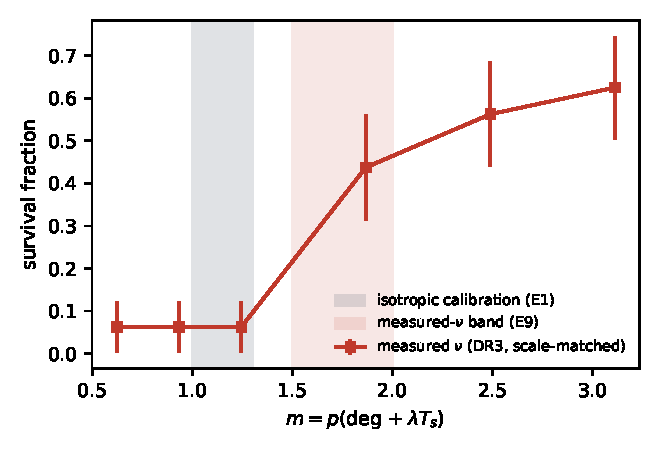
\includegraphics[width=.55\textwidth]{figs/fig5_e9.pdf}
\caption{実測 DR3 運動学上の生存閾値(等方較正と尺度整合): 閾値帯は約 1.5 倍
上方に移る。排除地図の保証レイヤは保守端($m>2.0$)を用いる。}
\label{fig:e9}
\end{figure}

\subsection{前線方向の感度}
前線族マーク場について、2種の事前分布(一様球/銀河中心バイアス)での方向平均の
差は $2.5\%$ --- 事前分布に頑健である。一方\textbf{方向ごと}のばらつきは大きい
($52\%$): 到来は向点集中するため、入植前線の効き目は太陽向点に対する前線方向に
依存する --- \cite{wright21} の入植方向論に接続する発見として報告する。

%======================================================================
\section{フライバイ網}\label{sec:flyby}

クリーン太陽通過の時変グラフ(ホライズン内 646 ノード、近日点状態は数値伝播で
抽出)の上で、憲法第3層の問いに答える: 推進剤最小の来訪経路は何か。任意の通過星に
搭乗した来訪者は、一本の弾道巡航脚で、近日点が太陽系深部に届く星へ乗り換えられる。
単一乗換の最小離脱予算は
\[
\Delta v \simeq 5.8\kms
\]
--- これは特定の星ではなく\textbf{網の統計的性質}である: 誤差 MC アンサンブルの
100\% で経路が存在し中央値 $5.7$--$5.9\kms$(離脱は全額推進剤 --- 共動する搭乗者は
フライバイで加速できない --- ゆえ予算は上界)。窓内の $0.1\pc$ 以内直接通過は
HD 7977 と GJ 710 で既知の記録と一致する。グラフ推定は定式化独立の対経路で検証
した: 実ポテンシャル中のヤコビアン・シューティングは 0.1 mpc 未満のミスに収束し、
乗換予算の変化は最大 $0.19\kms$(潮汐項は従属的)。多段最適化・全アンサンブル
再抽出・実恒星質量は網ファイル v1.1 に予約する。

\begin{figure}[t]\centering
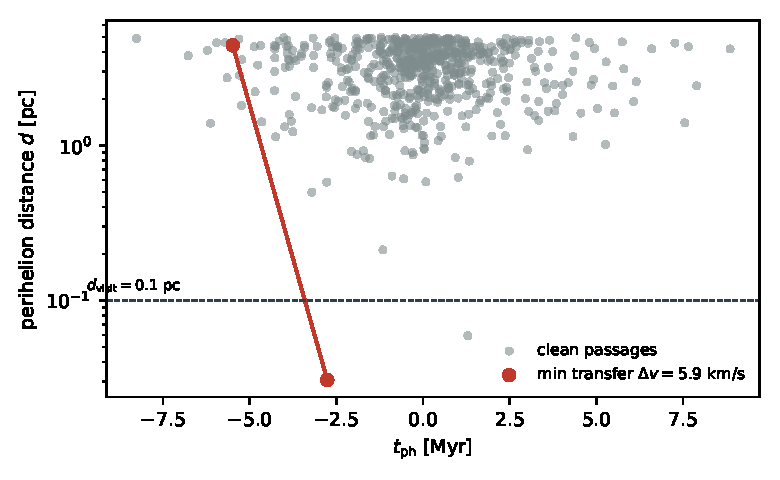
\includegraphics[width=.68\textwidth]{figs/fig3_flyby.pdf}
\caption{フライバイ網のノード集合(クリーン通過の近日点距離対時刻)と、
$d\le0.1\pc$ への最小単一乗換経路。}
\label{fig:flyby}
\end{figure}

%======================================================================
\section{議論}\label{sec:disc}

\textbf{判定不能の哲学。}アトラスの信頼性は非対称原理 --- 偽の判定可能より判定
不能 --- に立ち、3機構で実装される: 3成分の個別ホライズン(測定成長・ポテンシャル
乖離・予算型打切り)、両建て報告付きの5系統検疫、三値定理レイヤ。地図のどこも
沈黙裡の外挿では塗られていない。

\textbf{限界。}定理レイヤは実測速度分布の等方化近似の下で判定する(実分布は
非等方であり、E9 が誤差の向きを定量化する)。フライバイ網は太陽質量偏向体と単一
乗換を仮定する。1 pc 未満の $d^2$ 外挿と 5 pc 超はフラグ付きである。母集団は
FGK+早中期M であり、晩期M の来訪チャネルはここでは判定不能(率バウンド拡張は
予約)。

\textbf{公刊値との比較}は公刊会計規約の我々の再構成に基づく。本文から確定
できなかった点は付録Aに開示する。DR4 差替は設計段階から織り込まれている
(カタログは差替可能なデータ層である)。

%======================================================================
\section{結論}\label{sec:concl}

太陽近傍の実測運動学の上で、母集団と会計を宣言した上で: (1)クリーン到来率は
1 pc で $4.5^{+4.0}_{-2.7}\Myr^{-1}$ であり、公刊2倍分裂の主因は完備性対象母集団
の選択でデータ品質ではない。(2)標準航続距離で系の $0.5\%$ 超が入植済みなら
太陽系は過去 10\,Myr に訪問済みのはず --- その線より上で沈黙は 95\% の情報を持ち、
数学は長命な入植にのみ生存を保証するため、沈黙は長命入植を最も強く制約する。
(3)実恒星交通を通る推進剤最小の来訪経路が $\Delta v\simeq5.8\kms$ で常時存在
する。方法論的寄与は露出会計の分析、暗端 RV アーティファクト検疫と接線速度検査、
実測母集団橋付きの二帳簿完備性検査である。アトラスは測量であって証明ではない ---
しかし来訪の問いを、Gaia DR4 が研げる数字に変えた。

%======================================================================
\appendix

\section{GJ 710・公刊値分裂・再構成の限界}\label{app:gj710}
[英語版付録Aの訳出: GJ 710 の公刊値比較・単位換算仮説の中立記述・BJ+18/FP26 の
会計対照表全文と「公刊本文から確定できなかった12点」のリスト。]

\section{方法論記録と AI 開示}\label{app:method}
[英語版付録Bの訳出: 主張駆動の検証プロトコル・誤り台帳(G2 が発見した伝播精密化
欠陥2件、「一致している数字こそ疑え」の実話 = 相互に確認し合った 11.7 と 20.3 が
別々の理由で共に誤り)・AI システム(Claude Code, Claude Fable 5)の実行系として
の役割と人間の裁定・空の操舵介入ログ・内部検証は人間の査読の代替でないこと。]

\section{完備性地図のビン幅という隠れ正則化}\label{app:binwidth}
[英語版付録Cの訳出: 非単調走査($46.5\to23.7\to20.4\to27.1\to20.7\Myr^{-1}$)、
採用既定 $(1.5\Myr,0.75\pc)$+格子系統帯 $\pm15\%$、正準値併記。
図\ref{fig:binwidth}。]

\begin{figure}[t]\centering
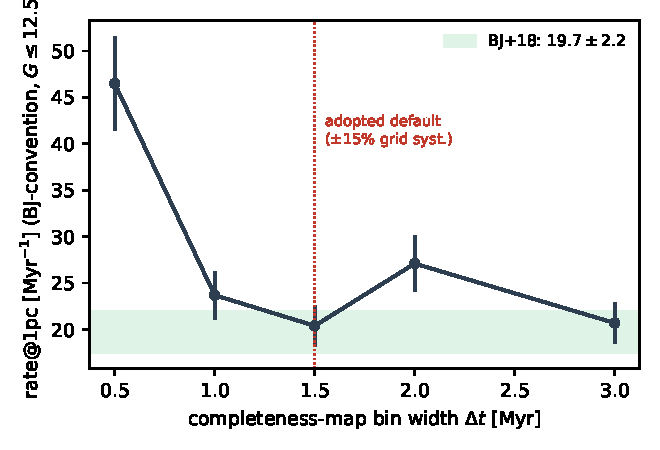
\includegraphics[width=.5\textwidth]{figs/fig4_binwidth.pdf}
\caption{モック完備性再構成率のビン幅走査: 隠れ正則化パラメータの開示。}
\label{fig:binwidth}
\end{figure}

\section{再現性とデータ公開}\label{app:release}
[英語版付録Dの訳出: 公開 JSON 3本+SHA-256 マニフェスト+全図表の再生成
コマンド+シミュレータ参照(追加互換スキーマ原則)。三点セット監査の論文側の錨。]

\bibliographystyle{plain}
\bibliography{wake_refs}

\end{document}
